\chapter{Design architetturale}\label{ch:design-architetturale}
A seguito dell'analisi dei requisiti definiti nel capitolo precedente, si è realizzato il design architetturale
di massima riportato in Figura~\ref{fig:architecture}.

I principali componenti individuati sono:
\begin{itemize}
    \item \texttt{World}: permette la registrazione e rimozione di \texttt{Entity} e \texttt{System}.
    Il metodo \texttt{update} rappresenta la principale modalità di aggiornamento dello stato di un~\texttt{World}: infatti, comporta la modifica dei \texttt{Component} delle \texttt{Entity} registrate secondo la logica descritta dai \texttt{System}.
    Inoltre, è possibile ottenere dal \texttt{World} delle \texttt{View} sulle \texttt{Entity} registrate
    \item \texttt{View}: permette di selezionare le \texttt{Entity} di un \texttt{World} che abbiano tutti i \texttt{Component} specificati
    \item \texttt{ExcludingView}: rappresenta una specializzazione di una \texttt{View} che permette di specificare un ulteriore filtro andando ad indicare i \texttt{Component} che una \texttt{Entity} non deve avere per essere parte della \texttt{View}
    \item \texttt{System}: descrive un'operazione che viene eseguita ogni volta che viene effettuata l'\texttt{update} del \texttt{World} in cui è registrato
    \item \texttt{IteratingSystem}: è un wrapper di una \texttt{View} che, indicando una specifica logica di aggiornamento, si occupa di iterare tutte le \texttt{Entity} selezionate aggiornandone i componenti
    \item \texttt{ExcludingSystem}: in maniera analoga a \texttt{IteratingSystem}, è un wrapper di una \texttt{ExcludingView}
    \item \texttt{Entity}: permette l'aggiunta e rimozione di \texttt{Component} e il loro aggiornamento.
    Non può trovarsi in più \texttt{World} contemporaneamente;
    mantiene un riferimento al \texttt{World} di appartenenza
    \item \texttt{Component}: descrive una particolare caratteristica di un'\texttt{Entity} alla quale viene aggiunto.
    Non può trovarsi in più di un'\texttt{Entity} contemporaneamente;
    mantiene un riferimento all'\texttt{Entity} di appartenenza
\end{itemize}

\begin{figure}[H]
    \centering
    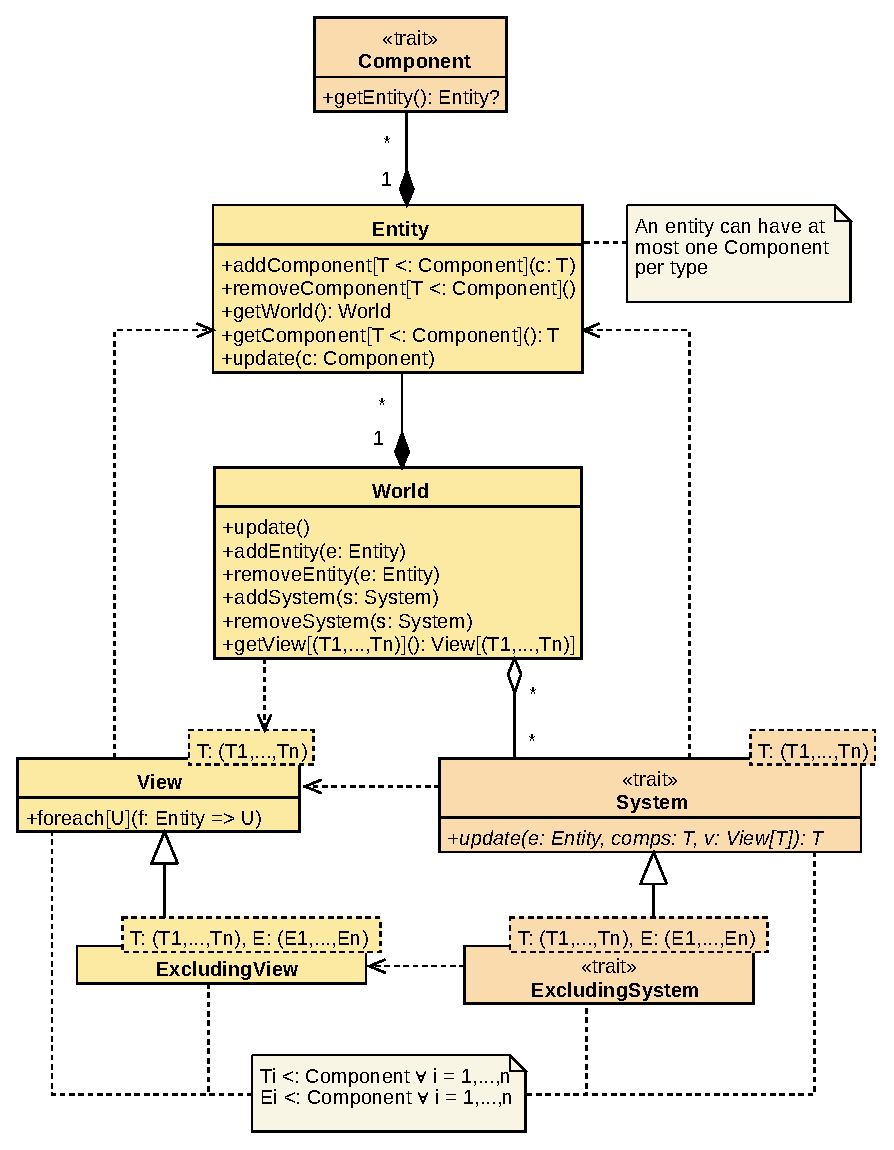
\includegraphics[width=\textwidth]{./img/Architechture}
    \caption{Diagramma delle classi rappresentante l'architettura del framework.}\label{fig:architecture}
\end{figure}

In Figura~\ref{fig:sequence} è riportato il diagramma di sequenza che descrive le principali interazioni che si
verificano quando viene effettuato l'\texttt{update} di un~\texttt{World}.

\begin{figure}[H]
    \centering
    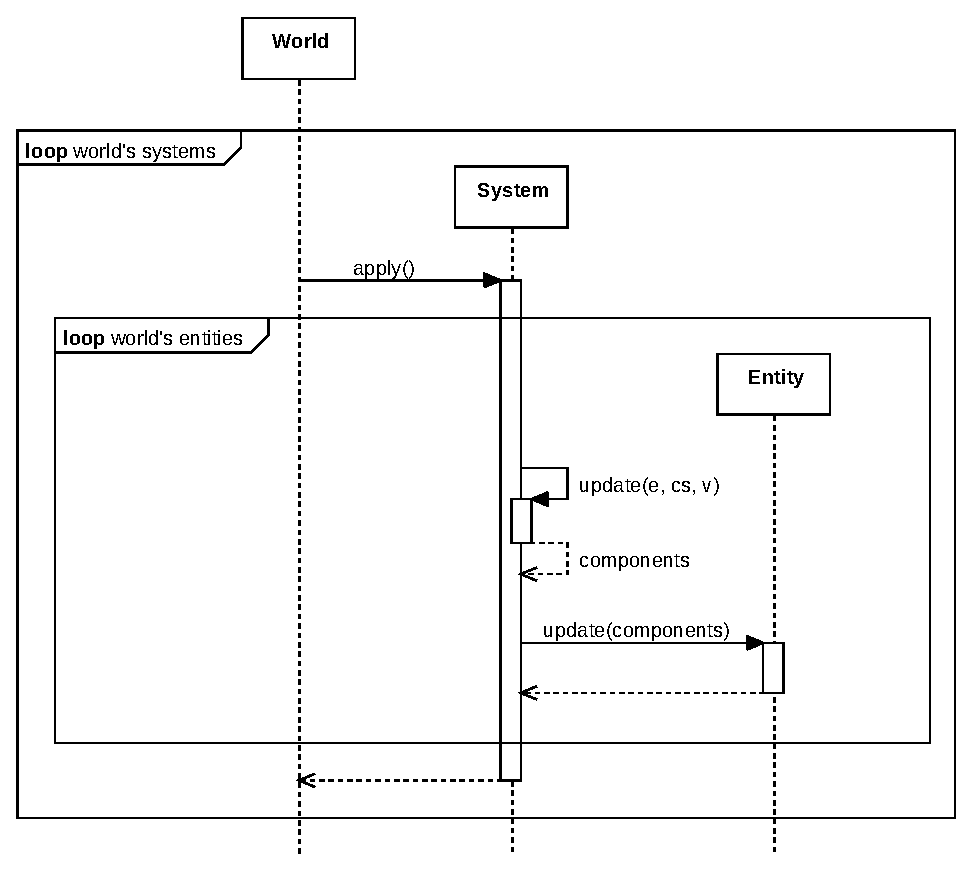
\includegraphics[width=\textwidth]{./img/Sequence}
    \caption{Diagramma di sequenza dell'aggiornamento dei componenti nel world.}\label{fig:sequence}
\end{figure}

Una volta aggiunti i \texttt{System} al~\texttt{World}, è possibile eseguirli affinché modifichino i componenti su cui
devono operare mediante la chiamata al metodo~\texttt{update}.
Per ogni sistema del world si verifica, tramite il metodo \texttt{shouldRun}, che questo possa essere eseguito.
In caso affermativo, il sistema viene eseguito chiamandone il metodo \texttt{update}.

L'esecuzione di ogni sistema è atomica e sequenziale: ciò significa che l'ordine con cui vengono inseriti nel
\texttt{World} è significativo ai fini della computazione degli stessi e non vi sono race condition.
